
%% version 0.0 Alpha
%% ronayumik@gmail.com
%% see airavata.me/about
%% for current contact information.

\documentclass[journal]{IEEEtran}
\usepackage{blindtext}
\usepackage{graphicx}
\usepackage{float}
\usepackage{hyperref}
\usepackage{nameref}
\usepackage{multirow}
\usepackage{graphicx}
\usepackage{array}
\usepackage{tabularx}
\usepackage{tabulary}
\usepackage{ltxtable} %for long table
\usepackage{etoolbox}
\usepackage{slantsc}
\usepackage{url}
\usepackage{booktabs}% http://ctan.org/pkg/booktabs
\let\labelindent\relax



% \let\author\relax % please?


\usepackage{enumitem}

\usepackage{caption}
% \usepackage{lon} %for long table

\usepackage{xcolor} %start packages for colored code listing
\usepackage{upquote} %start packages for colored code listing

% \usepackage{apacite} % for APA citing style
\usepackage{wrapfig} %untuk wrapfigure?
%reconfiguring inline list
\newlist{inlinelist}{enumerate*}{1}
\setlist*[inlinelist,1]{
	label={\alph*)},font={\color{red!50!black}\bfseries}
}

\hyphenation{op-tical net-works semi-conduc-tor}

\begin{document}
	
\title{Rancang Bangun Aplikasi \textit{web} Lelang \textit{Online} \textit{(E-Auction)} Berbasis Kerangka Kerja Laravel}{E-Auction Web Application Design and Implementation based on Laravel Framework}{KI141502} 

% \author{Nama Lengkap}{NRP}
\author{Ronauli Silva Natalensis Sidabukke}{5113100142}

% \supervisorOne{Nama Pembimbing Satu}{NIP}
% \supervisorTwo{Nama Pembimbing Dua}{NIP}
\supervisorOne{Rully Soelaiman, S.Kom, M.Kom}{197002131994021001}
\supervisorTwo{Rizky Januar Akbar, S.Kom., M.Eng}{198701032014041001}

% \degree{Nama Gelar}{Bidang Studi}{Program Studi}{Jurusan}{Jurusan (English)}{Fakultas}{Fakultas Singkatan}{Fakultas (English)}
\degree{Sarjana Komputer}{Algoritma Pemrograman}{S1}{Teknik Informatika}{Informatics}{Teknologi Informasi}{FTIf}{Information Technology}

% \time{bulan}{tahun}
\time{Juni}{2017}

	
	
\begin{abstract}
%\boldmath
\blindtext[1]
\end{abstract}
% IEEEtran.cls defaults to using nonbold math in the Abstract.

\begin{IEEEkeywords}
IEEEtran, journal, \LaTeX, paper, template.
\end{IEEEkeywords}

\IEEEpeerreviewmaketitle

	
\section{Pendahuluan}
Lelang adalah proses membeli dan menjual barang atau jasa dengan cara menawarkan kepada penawar, menawarkan tawaran harga lebih tinggi, dan kemudian menjual barang kepada penawar harga tertinggi\cite{balailelang_sejarah_nodate}. Transaksi jual beli saat ini sudah dapat dilakukan lewat berbagai cara, antara lain menggunakan \textit{e-commerce}, atau lewat \textit{social media}, atau bisa dengan melelang di aplikasi lelang \textit{online}. Sedikit berbeda dengan teknik penjualan di lelang online, karena aplikasi ini dapat diakses oleh banyak orang, tentu saja pelelang (\textit{auctioneer}) tidak terbatas pada ruang lelang saja, tapi bisa berasal dari manapun selama mereka mengakses aplikasi tersebut.  Lelang \textit{online} ini tentu saja mendatangkan banyak manfaat, selain biaya yang lebih efisien dan hemat, dan juga tidak menguras waktu karena siapapun, kapanpun, dimanapun dapat mengajukan penawaran ataupun melelang barangnya tanpa harus pergi ke instansi tertentu dan melakukan lelang dengan cara konvensional.\\
\indent Aplikasi serupa telah banyak, namun banyak aspek yang kurang dalam aplikasi tersebut, seperti informasi dari lelang tidak \textit{reliable} (misal: stok barang ternyata sudah habis), alur proses yang tidak jelas sehingga membingungkan pengguna aplikasi, informasi yang kurang jelas, dan produk yang didapatkan ternyata tidak sesuai dengan informasi pada saat produk dilelang (\textit{bad information}) \cite{ying-feng_kuo_online_2016}.\\
\indent Alur proses yang kurang diperhatikan oleh para developer aplikasi lelang \textit{online} menjadi beberapa alasan yang kuat mengapa lelang online masih kurang diminati \cite{noauthor_sistem_nodate}. Selain itu, bidang bisnis yang menuntut perubahan secara cepat tentu saja harus diadaptasi sehingga aplikasi bersifat fleksibel dengan \textit{maintainability} yang tinggi.

% \subsection{Subsection Heading Here}
% \blindtext

	
\section{Analisa dan Perancangan}
\subsection{\textit{Bussiness Engineering}}
Ketika bisnis digabungkan dengan teknologi atau yang sering disebut \textit{e-commerce}, hal yang sekedar pertukaran barang bertransformasi menjadi sebuah sistem interaktif yang kompleks dimana tujuan utamanya adalah menarik pengunjung/pengguna untuk menyelesaikan sebuah transaksi, yang berarti hanya memenuhi kebutuhan fungsional dasar saja tidak cukup - tapi juga bersifat \textit{well tailored to customers}\cite{bussiness_aspect_soft_eng}. Hal ini tentu sangat krusial, penting, dan tertantang untuk menyelesaikannya.

Dalam mencapai kesuksesan dan tingkat kompetitif yang tinggi, haruslah menyediakan layanan dengan kesan \textit{user experience (UX)} yang positif bagi para penggunanya. Fakta yang perlu diperhatikan dalam pengaruh \textit{user experience}, yaitu:
\begin{enumerate}[label=\alph*.]
	\item \textit{User tend to leave if a page loads more than 3 seconds};
	\item \textit{79\% of users won't return if the web's performance and experience is poor}; \textit{and}
	\item \textit{44\% of users will tell the poor experiences to their friends}\cite{georgiou_fast_2014}.
\end{enumerate}

\begin{figure}[H]
	\centering
	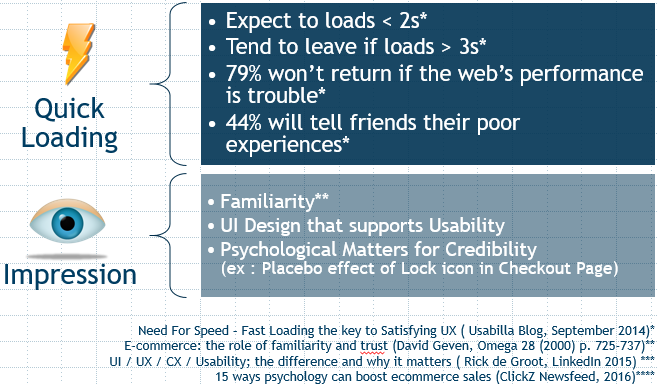
\includegraphics
	[width=.4\textwidth]
	{images/bab3/analisa/user-centered.png}
	\caption{Visualisasi aspek bisnis dalam \textit{software engineering}}
	\label{user-centered-analysis}
\end{figure}

Selain dari faktor \textit{user experience} dan \textit{performance}, beberapa hal yang menjadi poin penting dan menarik dalam beberapa studi yang terkait adalah sebagai berikut:
\begin{enumerate}[label=\alph*.]
	\item \textit{Familiarity} - yang dapat didefinisikan sebagai tingkat familier atau kesamaan dengan sistem sejenis ternyata dapat membangun \textit{trust} sehingga mensugesti pengguna untuk menyelesaikan transaksi yang dilakukan\cite{geven_e-commerce};
	\item \textit{Usability} yang memudahkan pengguna dalam menyelesaikan transaksi; dan
	\item Aspek-aspek psikologi seperti pemilihan warna, penggunaan \textit{icon} yang sesuai, seperti \textit{icon} gembok pada halaman pembayaran ternyata dapat mengesankan \textit{security} pada pengguna\cite{ewer_psychology_2014}\cite{coffin_color_2013}.
\end{enumerate}

\subsection{\textit{Technical Analysis}}
 Selain dari kualitas nilai jual aplikasi yang akan dibuat, ketahanan terhadap perubahan karena \textit{e-commerce} adalah sesuatu yang sangat cepat berubah karena kompetitor yang sangat kompetitif dan dorongan tehnologi yang membuat efektifitas dan efisiensi menjadi lebih baik.
Dari aspek \textit{software engineering} sendiri, \textit{software engineering} dimaksudkan untuk menunjang/\textit{support} pengembangan \textit{software} daripada \textit{individual programming}. Hal ini mencakup: \begin{inlinelist}
	\item \textit{evolution};
	\item \textit{design}; \textit{and}
	\item \textit{supporting program specification}
\end{inlinelist}\cite{software-engineering}.
Kebutuhan nonfungsional pada aplikasi ini didefinisikan pada Tabel 
%\captionsetup[table]{position=top,labelfont={sc},textfont={sl}}

\begin{table}[h!]
	\centering
	\caption{Kebutuhan Nonfungsional Aplikasi}
	\label{nonfung}
	\vfill
	\begin{tabular}{c|l|l}
		\hline
		\toprule
		No & Parameter & Keterangan\\ \hline
		\midrule
		1 & Ketersediaan & \textit{Available anytime via browser} \\ 
		2 & Bahasa & Menggunakan Bahasa Indonesia \\ 
		3 & Otorisasi & Otorisasi hak akses pengguna\\ 
		4 & Kecepatan & Waktu \textit{load} halaman kurang dari 3 detik \\ 
		5 & \textit{Positive User Experience} & Memberi kesan UX yang positif\\ 
		6 & \textit{Security} & Koneksi terlindung SSL/\textit{https}.\\ 
		7 & \textit{Maintainability} & Mudah di\textit{maintain}\\ 
		\bottomrule
	\end{tabular}
\end{table}

\subsection{Perancangan}	
	Sesuai definisi kebutuhan yang didefinisikan dalam \textit{paper}\cite{noauthor_application_2005}, kasus penggunaan aplikasi ini didefinisikan pada Gambar \ref{ucd.main}.
	\begin{figure}[h!]
		\centering
		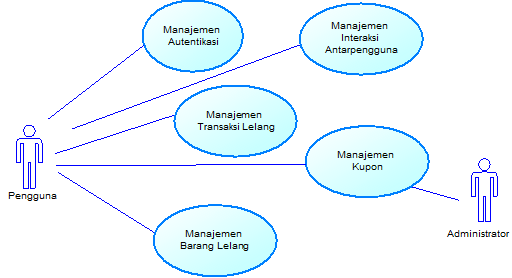
\includegraphics
		[width=.45\textwidth]
		{images/bab3/usecasediagram/ucd-main.png}
		\caption{Diagram Kasus Penggunaan Aplikasi}
		\label{ucd.main}
	\end{figure}
	Arsitektur fundamental diidentifikasi divisualisasikan pada Gambar \ref{fundamental-component} yaitu komponen-komponen penting dalam pembuatan aplikasi sebagai berikut.
	\begin{enumerate}
		\item Web Server 
		\item Mekanisme penyimpanan data (\textit{database} dan \textit{data storage})
		\item \textit{User Interface} sebagai media terhadap \textit{end-user}
		\item Mekanisme Asinkronus untuk mengakomodasi fitur \textit{realtime}
	\end{enumerate}
	
	\begin{figure}[h!]
		\centering
		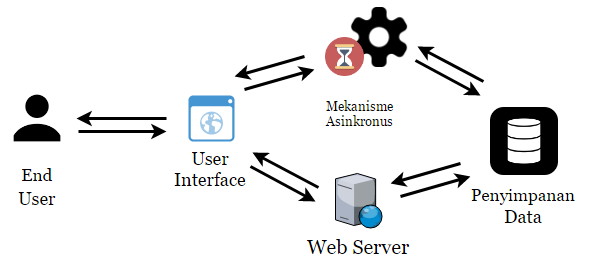
\includegraphics
		[width=.45\textwidth]
		{images/bab3/buku/basic_architecture.png}
		\caption{Arsitektur dasar yang dibutuhkan untuk membangun aplikasi}
		\label{fundamental-component}
	\end{figure}
	
	Digabungkan dengan kebutuhan fungsionalitas dan kelebihan kekurangan masing-masing teknologi pembangun yang ada, maka didefinisikan arsitektur lengkap dan pemilihan teknologi seperti pada gambar \ref{final-arch-tech-figure}.
	
	\begin{figure}[H]
		\centering
		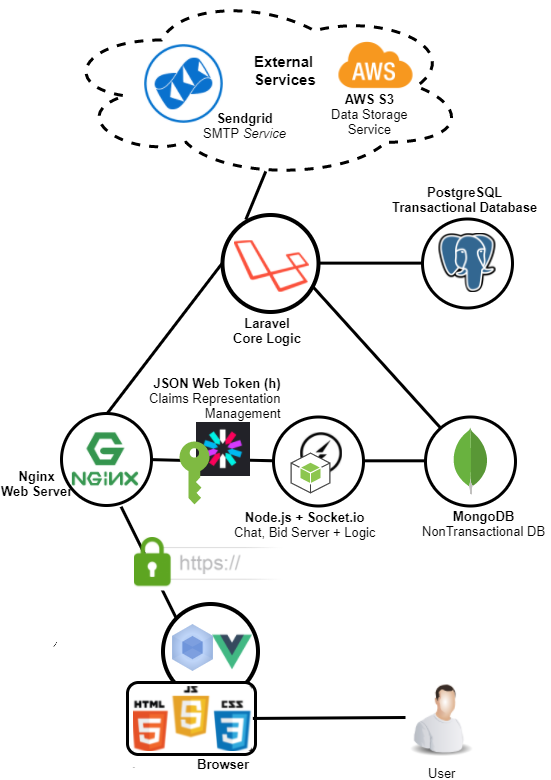
\includegraphics[width=.4\textwidth]{images/bab3/diagram-portrait.png}
		\caption{Visualisasi arsitektur dan teknologi Final yang diterapkan dalam rancang bangun aplikasi}
		\label{final-arch-tech-figure}
	\end{figure}
	
		
		Untuk mengakomodasi kebutuhan \textit{flexibility} dan \textit{maintainability}, maka penulis membangun aplikasi dengan menggunakan \textit{repository} pattern, dengan pembagian lingkup \textit{tiers} sebagai berikut:
		\begin{enumerate}
			\item \textit{Presentation tier}, bertanggungjawab terhadap tampilan dan \textit{view logic} di lingkup \textit{browser} pengguna;
			\item \textit{Bussiness tier}, merupakan \textit{logic} dari proses bisnis aplikasi;
			\item \textit{Integration tier}, merupakan integrasi manajemen pemrosesan data dan \textit{external services}; dan
			\item \textit{Resource tier}, bertanggung jawab terhadap \textit{data access layer}.
		\end{enumerate}
		\begin{figure}[]
			\centering
			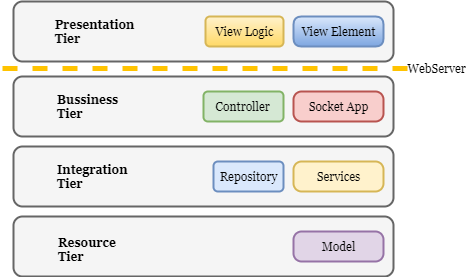
\includegraphics[width=.4\textwidth]{images/bab3/apl/main-apl.png}
			\caption{Visualisasi arsitektur dan teknologi Final yang diterapkan dalam rancang bangun aplikasi}
			\label{tiers}
		\end{figure}
\subsection{Deskripsi Sistem}
Aplikasi dapat diakses melalui \textit{browser} lewat URL {\url{https://lelangapa.com}}. Seperti \textit{e-commerce} pada umumnya, siapa saja dapat mendaftar ke dalam sistem sebagai dan memulai aktivitas lelang, baik sebagai pelelang maupun penjual barang.
\begin{figure}[h!]
	\centering
	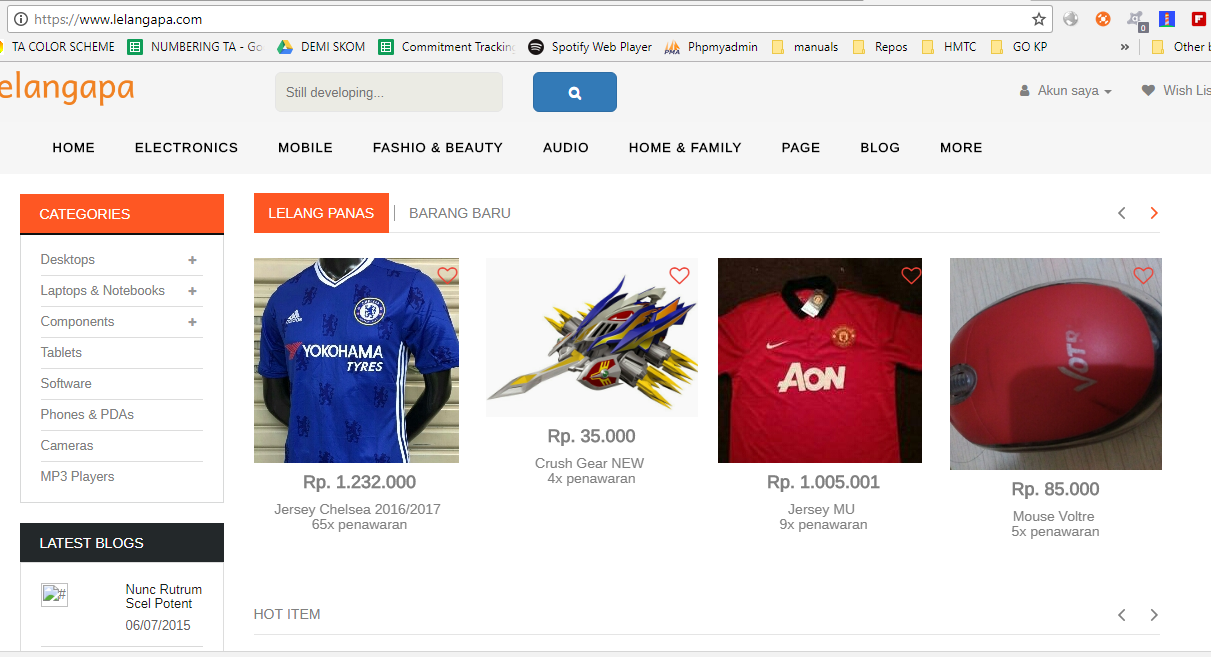
\includegraphics[width=.45\textwidth]{images/UI/landing.png}
	\caption{Tampilan \textit{landing page} aplikasi}
	\label{snap-landing}
\end{figure}

	% si deskripsi sistem masuk subsistem sebelumnya
	% jadi subsection
	\input{deskripsi-sistem}
%	
\section{Deskripsi Aplikasi}


\subsection{Subsection Heading Here}
\blindtext

	\section{Pengujian \& Evaluasi}

\subsection{Kecepatan Sistem}
Pengujian kecepatan dilakukan dengan menggunakan Google Chrome Developer Tools, dimana untuk setiap kasus penggunaan diuji dengan segmentasi \textit{loading time} sebagai berikut \begin{inlinelist}
	\item \textit{DOM Loading}
	\item \textit{Scripting}
	\item \textit{Rendering}
\end{inlinelist}. Rata-rata keseluruhan \textit{loading page} adalah 3,2 detik (lebih 6\% dari target). Untuk menganalisa dengan visualisasi masing-masing segmen pada Gambar \ref{bar-chart-speed}.
\begin{figure}[b]
	\centering
	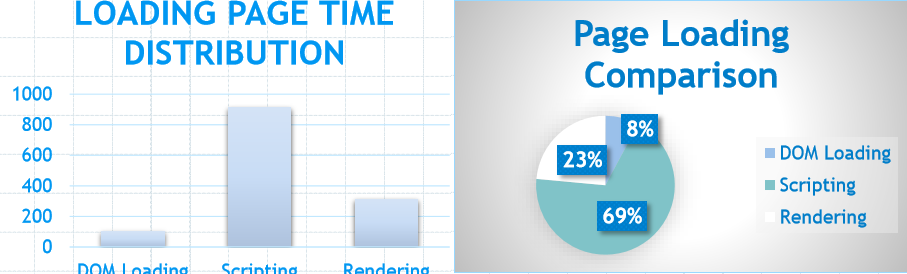
\includegraphics[width=.4\textwidth]{images/bab5/speed/combined.png}
	\caption{Diagram Visualisasi dan Perbandingan Waktu per Segmen}
	\label{bar-chart-speed}
\end{figure}
	Dengan menggunakan \textit{tool} Lighthouse, \textit{scripting} memakan waktu yang sangat besar (hampir 75|\% \textit{loading time}) untuk \textit{loading} gambar, yang ternyata ini menjadi masalah umum pada website \textit{e-commerce}, dimana penyelesaiannya menggunakan teknik \textit{image optimization}.

\subsection{\textit{Maintainability Assesment}}
Pengujian \textit{maintainability} dilakukan dengan mengikuti pedoman dari paper "A Software Maintainability Evaluation Methodology"\cite{peercy_software_nodate}, yaitu parameter utama: \textit{modularity}, \textit{descriptiveness}, \textit{consistency}, \textit{simplicity}, dan \textit{trackability}. Sesuai dengan paper tersebut, dengan dua aspek penilaian - kode sumber dan dokumentasi sistem dengan \textit{weight} masing-masing yang berbeda - rekapitulasi hasil dapat dilihat pada Gambar \ref{maintainability-recap}.

\begin{table}[h]
	\centering
	\caption{Rekapitulasi Pengujian \textit{Maintainability Assesment}}
	\label{maintainability-recap}
	\begin{tabular}{c|c|c|c}
		\toprule
		\textbf{Parameter} & \textbf{Kode Sumber} & \textbf{Dokumentasi Sistem} & \textbf{Rata-rata} \\
		\hline
		
		\textit{Modularity} & 83\% & 83\% & 83\% \\ 
		\textit{Descriptiveness} & 83\% & 78\% & 80\% \\ 
		\textit{Consistency} & 78\% & 73\% & 75\% \\ 
		\textit{Simplicity} & 75\% & 73\% & 74\% \\ 
		\textit{Trackability} & 75\% & 73\% & 77\% \\ 
		Rata-rata & 79\% & 76\% &  \\ 
		\textit{weight} & 0.6 & 0.4 &  \\ \hline
		\textbf{Skor} & \multicolumn{3}{|c}{77\% (pencapaian 96\%)} \\ \hline
	\end{tabular}
\end{table}

\subsection{\textit{User Experience Assesment}}
Pengujian \textit{maintainability} dilakukan dengan mengikuti pedoman dari paper " Development of an Instrument Measuring User Satisfaction of the Human-Computer Interface"\cite{chin_development_1998}. Rekapitulasi hasil dapat dilihat pada Tabel \ref{ux-recap}, dan visualisasi hasil berbentuk diagram dapat dilihat pada Gambar \ref{ux-chart}.

\begin{table}[t]
	\centering
	\caption{Rekapitulasi Hasil \textit{User Experience Assesment}}
	\label{ux-recap}
	\vfill
	\begin{tabular}{c|c|c|c}
		\hline
		\toprule
		\textbf{\begin{tabular}[c]{@{}c@{}}Parameter/\\ Kriteria\end{tabular}} & \textbf{\begin{tabular}[c]{@{}c@{}}Skor\\ Aplikasi Lain\end{tabular}} & \textbf{\begin{tabular}[c]{@{}c@{}}Skor\\ Aplikasi Lelangapa\end{tabular}} & \textbf{\begin{tabular}[c]{@{}c@{}}Persentase\\ Perbedaan\end{tabular}} \\ \hline
		
		\midrule
		
		\begin{tabular}[c]{@{}c@{}}Desain\\ \& Impresi Web\end{tabular} & 3.3 & 4.1 & +20\% \\ 
		\begin{tabular}[c]{@{}c@{}}Konsistensi\\ \& Descriptiveness\end{tabular} & 3.5 & 4.2 & +17\% \\ 
		\textit{Easiness} & 3.1 & 3.9 & +21\% \\ 
		\textit{\begin{tabular}[c]{@{}c@{}}Clear \\ Error Messages\end{tabular}} & 3.7 & 3.9 & +5\% \\ 
		\textit{\begin{tabular}[c]{@{}c@{}}Clear\\ Status Process\end{tabular}} & 3.3 & 4 & +18\% \\ 
		\textit{Performance} & 3.7 & 3.8 & +3\% \\ 
		\begin{tabular}[c]{@{}c@{}}Penilaian\\ Keseluruhan\end{tabular} & 3.7 & 4.3 & +14\% \\ 
		\begin{tabular}[c]{@{}c@{}}Rekomendasi\\ pada Teman?\end{tabular} & 3.4 & 4.0 & +15\% \\ \hline
		\multicolumn{3}{c}{\textbf{Total Rata-rata Keseluruhan}} & \multicolumn{1}{c}{+15\%} \\ 
		
		\bottomrule
	\end{tabular}
\end{table}

\begin{figure}[b]
	\centering
	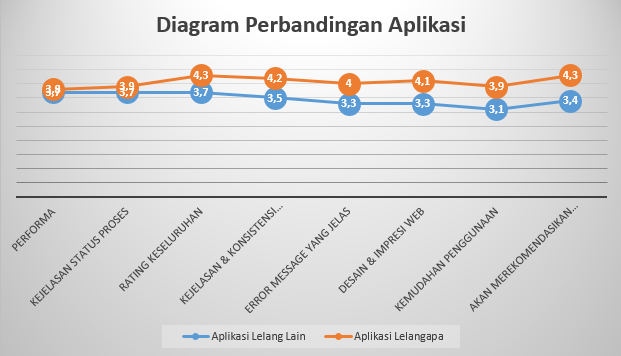
\includegraphics[width=.4\textwidth]{images/bab5/ujipengguna/chart.png}
	\caption{Visualisasi Perbandingan Hasil \textit{User Experience Assesment} Aplikasi dengan Aplikasi Lainnya}
	\label{ux-chart}
\end{figure}



	%
\section{Introduction}
\blindtext

\subsection{Subsection Heading Here}
\blindtext

	
\section{Kesimpulan}
Dari hasil pengamatan selama proses perancangan hasil uji coba yang telah dilakukan terhadap sistem yang dikembangkan, diambil kesimpulan sebagai berikut:
\begin{enumerate}
	\item \textit{Software design} adalah tahap yang sangat penting dan harus dibuat sefleksibel mungkin mengingat \textit{e-commerce} adalah bisnis menuntut perubahan yang cepat, sehingga agar tidak tersaingi kompetitor, harus dirancang sedemikian rupa agar perubahan tersebut dapat diimplementasi tanpa \textit{cost} (misal \textit{refactoring}) yang besar.
	\item Aspek dan \textit{advices} bisnis sangat penting dalam membuat aplikasi \textit{e-commerce}, dimana \textit{well-tailored to customer application}-lah yang dapat memenangkan pasar. Oleh karena itu, sangat penting untuk meninjau aspek \textit{usability} dan \textit{user experience} agar memberi kesan positif pada pengguna, dan pengguna tetap mau bertransaksi kembali dalam aplikasi tersebut.
\end{enumerate}

Pengembangan yang dapat dilakukan berikutnya yaitu dengan:
\begin{enumerate}
	\item \textit{Image Optimization} agar \textit{loading time} dapat dikurangi, dan meningkatkan \textit{user experience} dalam aspek \textit{application performance};
	\item \textit{Advanced data management \& searching}, dimana \textit{data growth} dalam \textit{e-commerce} sangatlah masif sehingga dibutuhkan teknik khusus lebih dari sekedar \textit{query}; dan
	\item \textit{Market Engagement} - menjaga \textit{market} yang telah dibangun dengan menggunakan pendekatan statistik atau \textit{machine learning}, dapat dilakukan \textit{customer scoring} dan \textit{early fraud detection} lewat analisa riwayat transaksi pengguna. Dengan \textit{score} tersebut, kita dapat merekomendasikan barang-barang yang sesuai dengan pengguna dan \textit{early-fraud detection} untuk menciptakan lingkungan lelang yang lebih aman dan terpercaya pada pengguna.
\end{enumerate}
	%	
\appendices
\section{Proof of the First Zonklar Equation}
Some text for the appendix.

	% % use section* for acknowledgement
\section*{Ucapan Terima Kasih}
Penulis menghaturkan terimakasih yang sebesar-besarnya kepada dosen pembimbing yang berbaik hati memantau dan memberikan saran bimbingan pengerjaan penelitian ini, Andre sebagai partner satu topik untuk berdiskusi dalam pemecahan masalah, orangtua penulis yang selalu memberi \textit{support}, serta pihak-pihak lain yang tidak disebutkan dan telah membantu dalam pengerjaan penelitian ini.

\ifCLASSOPTIONcaptionsoff
  \newpage
\fi

	\bibliography{Zotero}
	\bibliographystyle{ieeetran}
	%
\begin{IEEEbiography}[{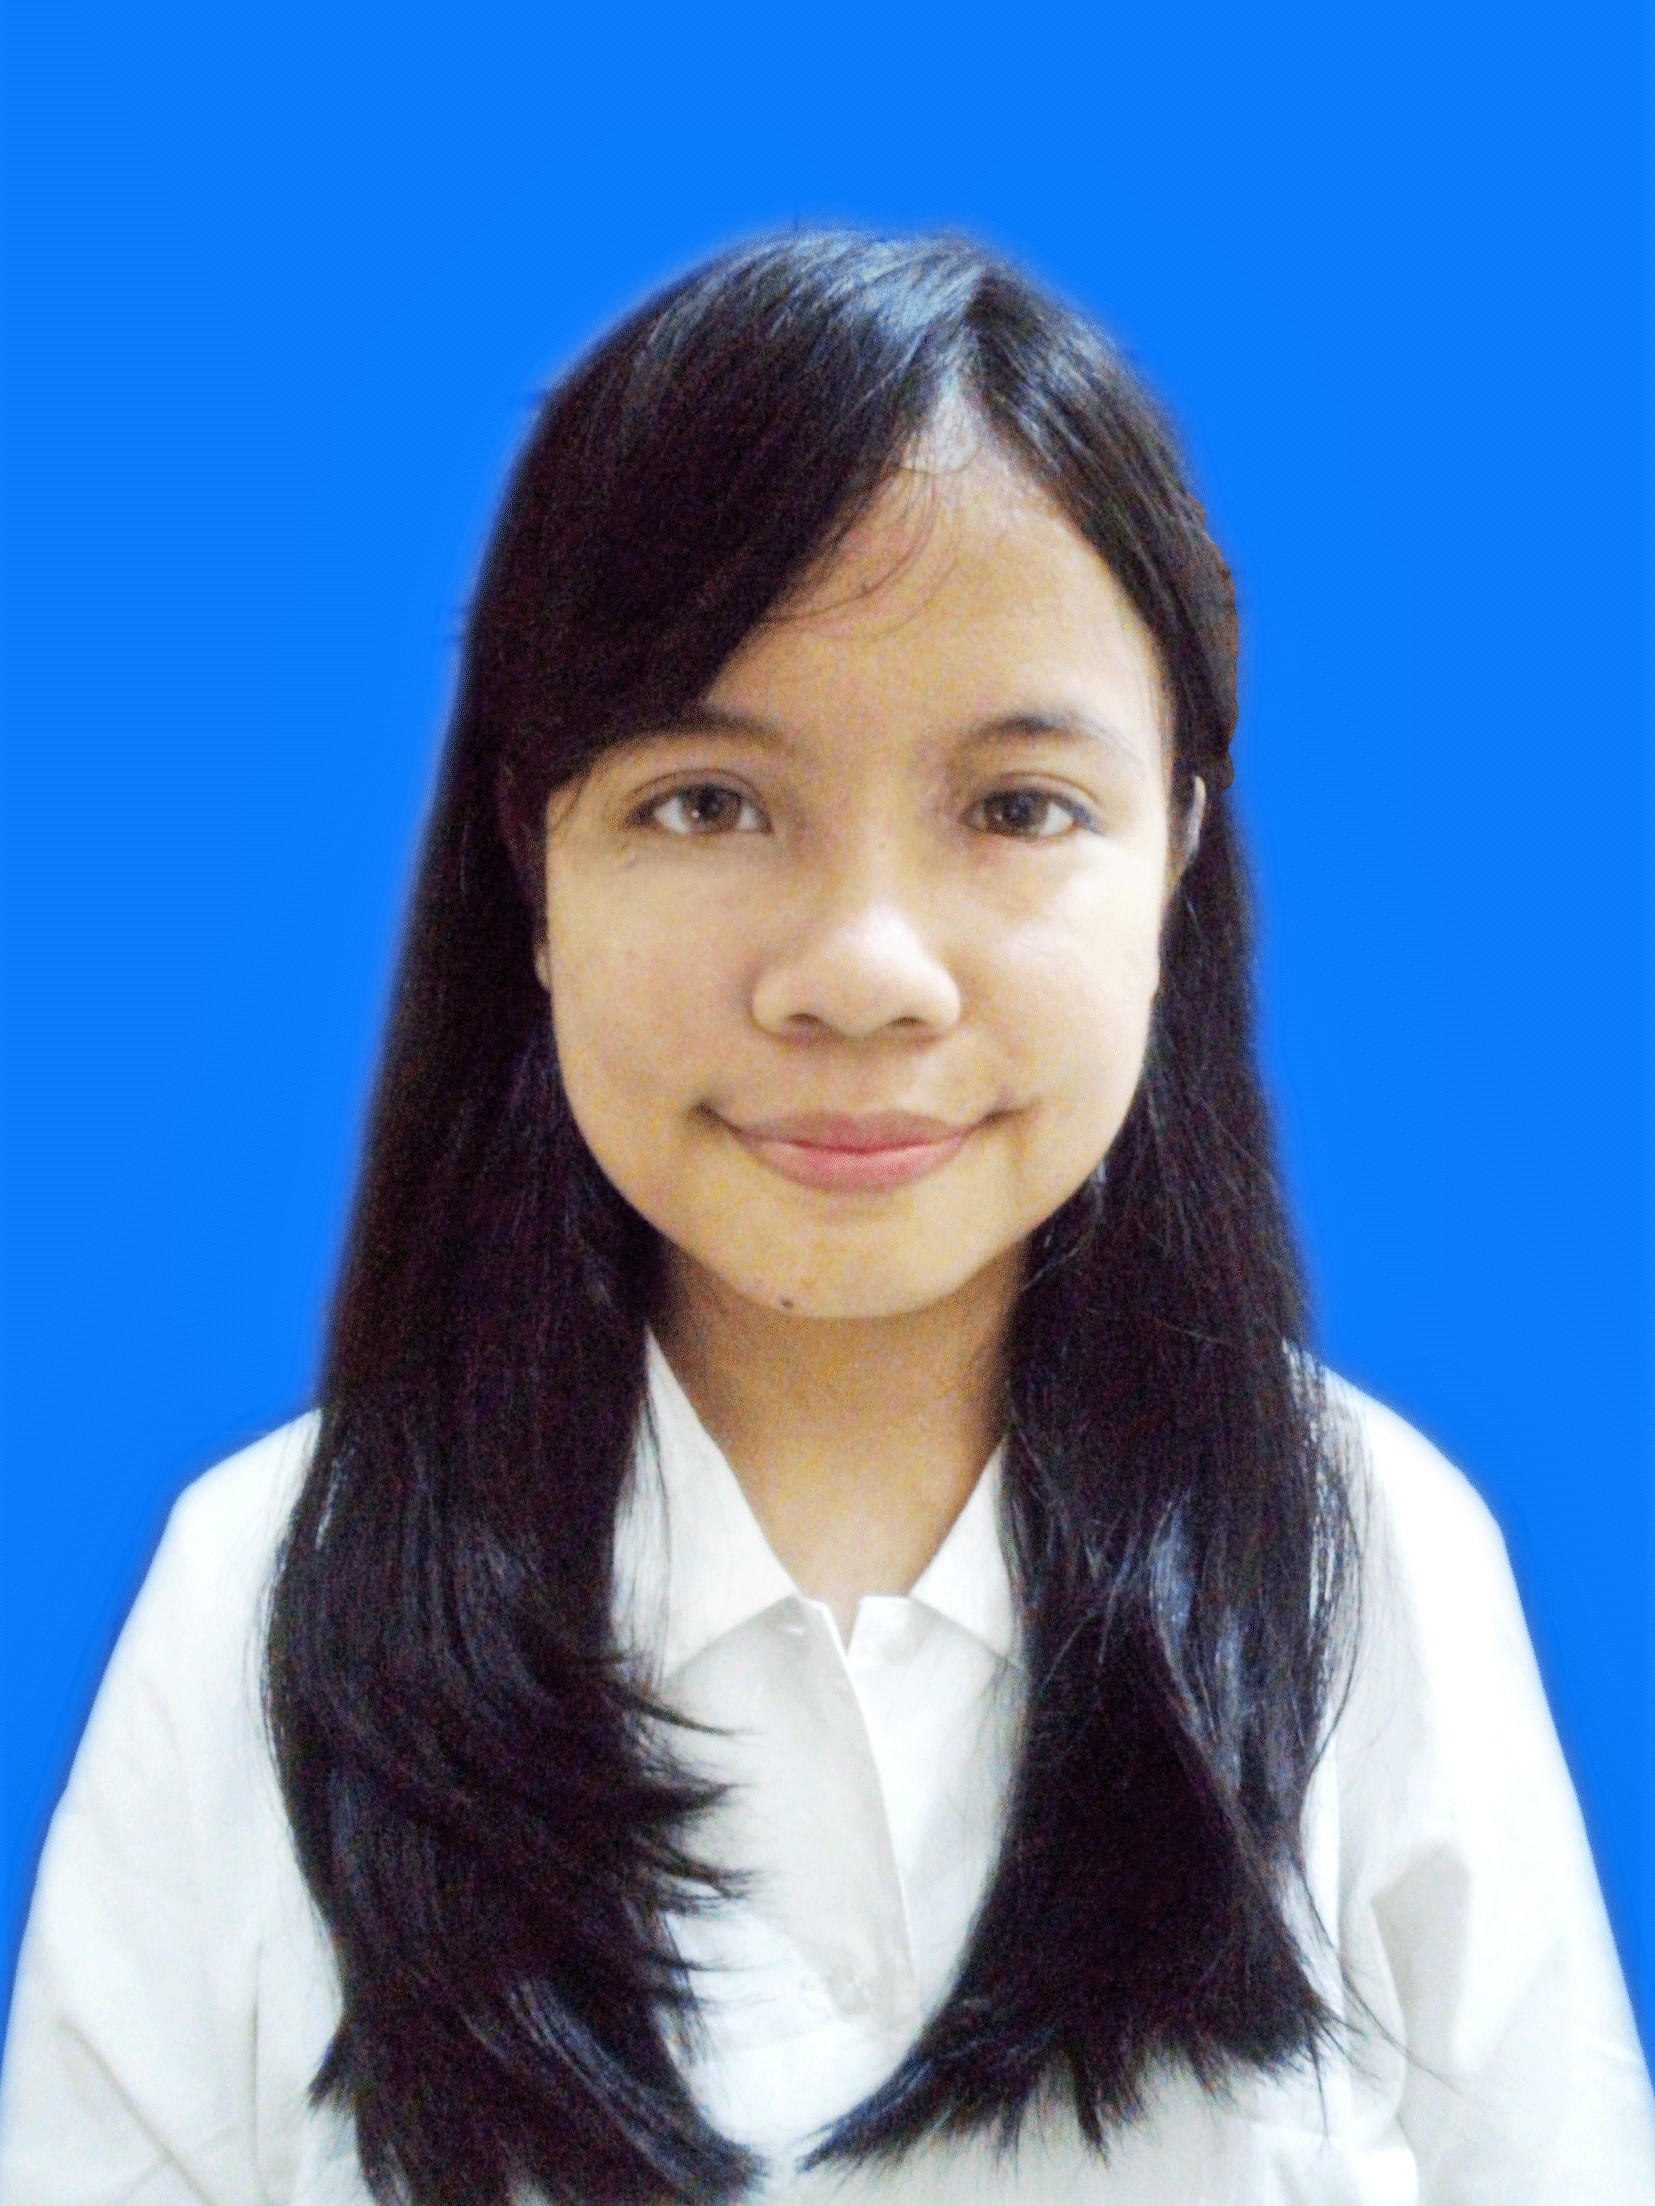
\includegraphics[width=1in,height=1.25in,clip,keepaspectratio]{picture}}]{John Doe}
\blindtext
\end{IEEEbiography}
% let's finish this
% happily
\end{document}


